% Classes of src/core/Math/Interpolation and their dependencies. Paper: section "Interpolation, integration and
% differentiation" (fig:interpolation); Doxygen: Interpolation.hpp.
%   pdflatex InterpolationClasses.tex; pdftoppm -r 200 -png -singlefile InterpolationClasses.pdf InterpolationClasses;
%   pdftocairo -svg InterpolationClasses.pdf InterpolationClasses.svg
\documentclass[tikz,border=2pt]{standalone}
% Shared style of the class diagrams of CAP (figures/*Classes.tex): \input after \documentclass[tikz]{standalone}.
%  - boxes: blue = abstract base class, light blue = class, green = entry class of the folder (steering class, task),
%    yellow = free functions (tools), grey = class of another folder;
%  - arrows: open triangle = inherits from; dashed with diamond = owns (holds); dashed with arrow = uses.
\usepackage[scaled=0.92]{helvet}
\usetikzlibrary{arrows.meta,shapes.multipart,positioning,fit,backgrounds,calc}
\renewcommand{\familydefault}{\sfdefault}
\definecolor{abstract}{HTML}{D6E4F5}
\definecolor{concrete}{HTML}{EEF4FB}
\definecolor{steer}{HTML}{DCEFD9}
\definecolor{tools}{HTML}{FFF8E6}
\definecolor{external}{HTML}{E9E9E9}
\definecolor{dependline}{HTML}{8A6D3B}
\definecolor{folder}{HTML}{F7F7F7}
\tikzset{
  every picture/.style={font=\scriptsize},
  cls/.style={draw, fill=concrete, align=center, inner sep=2.5pt, text width=#1, font=\tiny},
  cls/.default=3.0cm,
  abs/.style={cls=#1, fill=abstract},
  abs/.default=3.0cm,
  steer/.style={cls=#1, fill=steer, line width=0.8pt},
  steer/.default=4.2cm,
  tool/.style={cls=#1, fill=tools},
  tool/.default=4.2cm,
  ext/.style={cls=#1, fill=external, dashed},
  ext/.default=2.6cm,
  fam/.style={draw, rectangle split, rectangle split parts=2, rectangle split part fill={#1,white},
              rectangle split part align={center,left}, inner sep=2.5pt, align=left},
  inherit/.style={-{Triangle[open,length=2.2mm,width=2.2mm]}, thin},
  uses/.style={dashed, dependline, -{Stealth[length=1.6mm]}, thin},
  owns/.style={dashed, dependline, {Diamond[length=2.4mm,width=1.6mm]}-, thin},
  lbl/.style={font=\tiny, text=dependline, align=center},
  note/.style={font=\tiny, align=left, text=black!70},
  title/.style={font=\footnotesize\bfseries, anchor=north west},
}
% a member line in a class box
\newcommand{\m}[1]{\\#1}
\newcommand{\cn}[1]{{\scriptsize\textbf{#1}}}
\newcommand{\an}[1]{{\scriptsize\textbf{\textit{#1}}}}

% legend common to the class diagrams (place with \legendat{x}{y})
\newcommand{\legendat}[2]{%
  \begin{scope}[shift={(#1,#2)}, font=\tiny]
    \node[abs=0.9cm, minimum height=3mm, inner sep=1pt] (lA) at (0,0) {abstract};
    \node[cls=0.9cm, minimum height=3mm, inner sep=1pt, right=1mm of lA] (lC) {class};
    \node[steer=1.1cm, minimum height=3mm, inner sep=1pt, right=1mm of lC] (lS) {entry class};
    \node[tool=1.1cm, minimum height=3mm, inner sep=1pt, right=1mm of lS] (lT) {functions};
    \node[ext=1.3cm, minimum height=3mm, inner sep=1pt, right=1mm of lT] (lE) {other folder};
    \draw[inherit] ($(lE.east)+(1mm,0)$) -- ++(5mm,0) node[right, inner sep=1pt] (l1) {inherits};
    \draw[owns] ($(l1.east)+(1mm,0)$) -- ++(5mm,0) node[right, inner sep=1pt] (l2) {owns};
    \draw[uses] ($(l2.east)+(1mm,0)$) -- ++(5mm,0) node[right, inner sep=1pt] {uses};
  \end{scope}}

\begin{document}
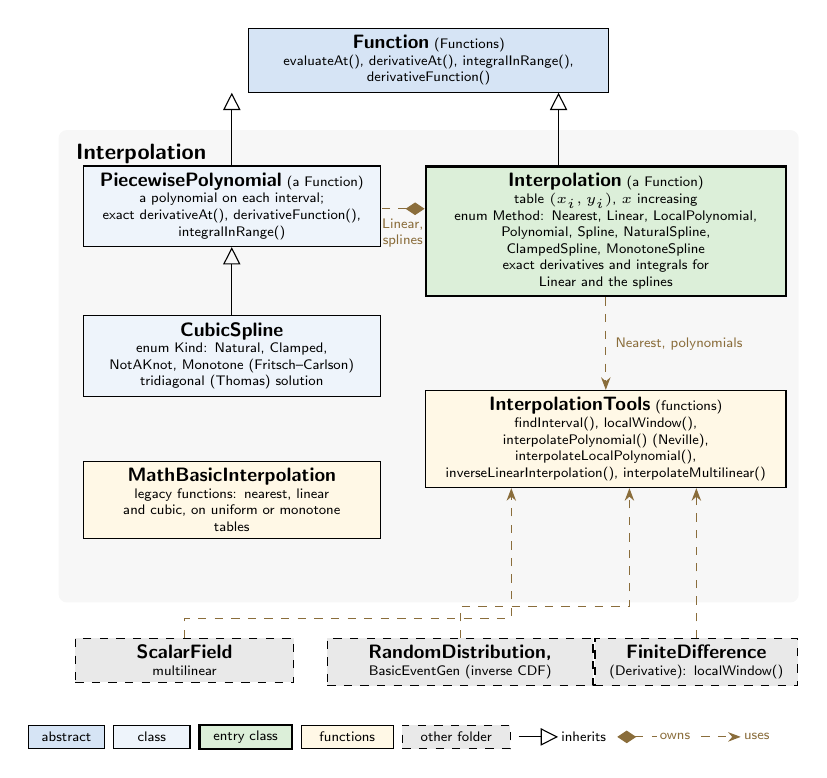
\begin{tikzpicture}[every node/.append style={anchor=north}]
  \begin{scope}[on background layer]
    \fill[folder, rounded corners=3pt] (-0.1,-1.0) rectangle (9.3,-7.0);
  \end{scope}
  \node[title] at (0.0,-1.05) {Interpolation};

  \node[abs=4.4cm] (Function) at (4.6,0.3)
    {\an{Function} \tiny(Functions)\m{evaluateAt(), derivativeAt(), integralInRange(),}\m{derivativeFunction()}};

  \node[steer=4.4cm] (Interp) at (6.85,-1.45)
    {\cn{Interpolation} \tiny(a Function)\m{table $(x_i, y_i)$, $x$ increasing}
     \m{enum Method: Nearest, Linear, LocalPolynomial,}\m{Polynomial, Spline, NaturalSpline,}
     \m{ClampedSpline, MonotoneSpline}\m{exact derivatives and integrals for}\m{Linear and the splines}};
  \node[cls=3.6cm] (PP) at (2.1,-1.45)
    {\cn{PiecewisePolynomial} \tiny(a Function)\m{a polynomial on each interval;}
     \m{exact derivativeAt(), derivativeFunction(),}\m{integralInRange()}};
  \node[cls=3.6cm] (CS) at (2.1,-3.35)
    {\cn{CubicSpline}\m{enum Kind: Natural, Clamped,}\m{NotAKnot, Monotone (Fritsch--Carlson)}
     \m{tridiagonal (Thomas) solution}};
  \node[tool=4.4cm] (Tools) at (6.85,-4.3)
    {\cn{InterpolationTools} \tiny(functions)\m{findInterval(), localWindow(),}
     \m{interpolatePolynomial() (Neville),}\m{interpolateLocalPolynomial(),}
     \m{inverseLinearInterpolation(), interpolateMultilinear()}};
  \node[tool=3.6cm] (Basic) at (2.1,-5.2)
    {\cn{MathBasicInterpolation}\m{legacy functions: nearest, linear}\m{and cubic, on uniform or monotone}\m{tables}};

  \draw[inherit] (PP.north) -- (PP.north |- Function.south);
  \draw[inherit] ([xshift=-0.6cm]Interp.north) -- ([xshift=-0.6cm]Interp.north |- Function.south);
  \draw[inherit] (CS.north) -- (PP.south);
  \draw[owns] (Interp.west |- 0,-2.0) -- node[lbl, below]{Linear,\\splines} (PP.east |- 0,-2.0);
  \draw[uses] (Interp.south) -- node[lbl, right]{Nearest, polynomials} (Tools.north);

  \node[ext=2.6cm] (Field) at (1.5,-7.45) {\cn{ScalarField}\m{multilinear}};
  \node[ext=3.2cm] (RD) at (5.0,-7.45) {\cn{RandomDistribution,}\m{BasicEventGen (inverse CDF)}};
  \node[ext=2.4cm] (Plot) at (8.0,-7.45) {\cn{FiniteDifference}\m{(Derivative): localWindow()}};
  \draw[uses] (Field.north) -- ++(0,0.25) -| ([xshift=-1.2cm]Tools.south);
  \draw[uses] (RD.north) -- ++(0,0.4) -| ([xshift=0.3cm]Tools.south);
  \draw[uses] (Plot.north) -- (Plot.north |- Tools.south);
  \legendat{0.0}{-8.55}
\end{tikzpicture}
\end{document}
